\section{ASSEMBLY}
\label{sec:Assembly}

\begin{figure}[ht]
\begin{center}
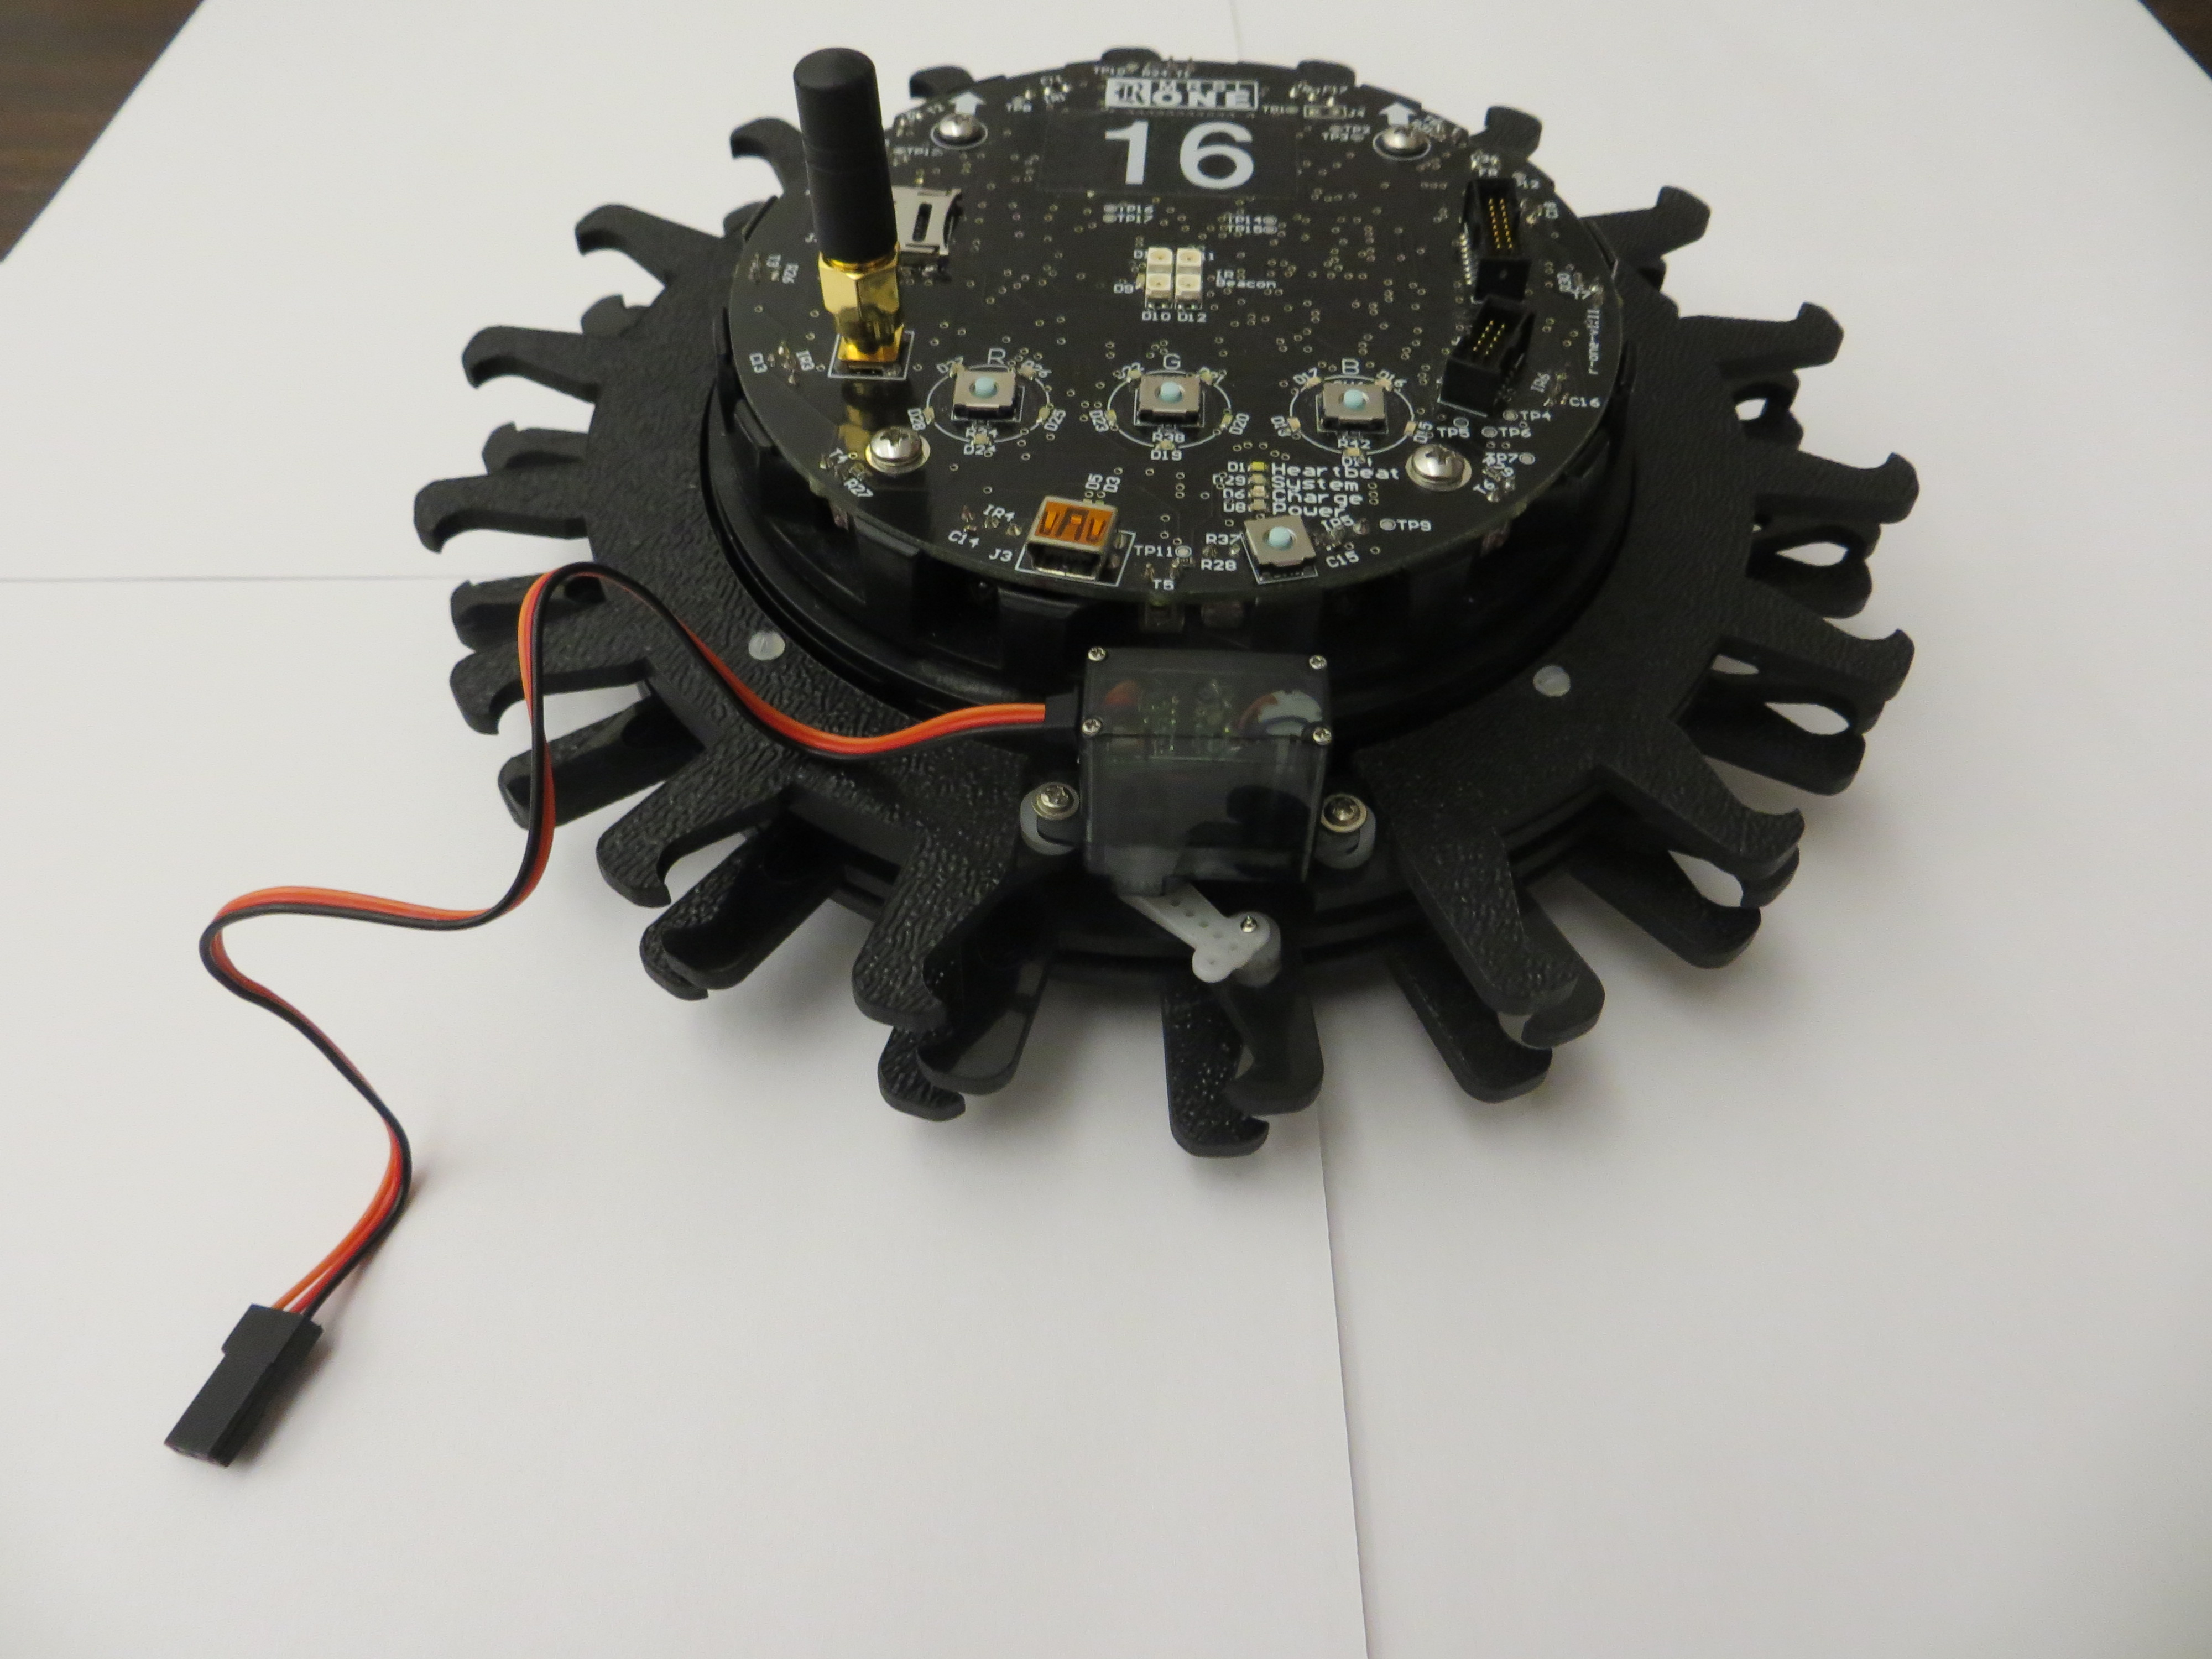
\includegraphics[width=.5\linewidth]{./Figs/back_closed}
\end{center}
\caption{}
\label{fig:back closed}
\end{figure}

There are many different components that go into the R-One Manipulator. A couple of them are just improvements over the last iteration of manipulator, the Velcro skirt, and others had to be specially designed for the purpose of the actuated manipulator. 

All of these components are laser cut from 1/8th inch ABS plastic. However, this is an option that can be reviewed for the best possible material to use. 

The servo used was pulled from the servo bin in the lab, and should be easily replaced. However, it may be beneficial for future use to find the smallest possible servo to minimize space requirements. 

\begin{figure}[h]
\begin{center}
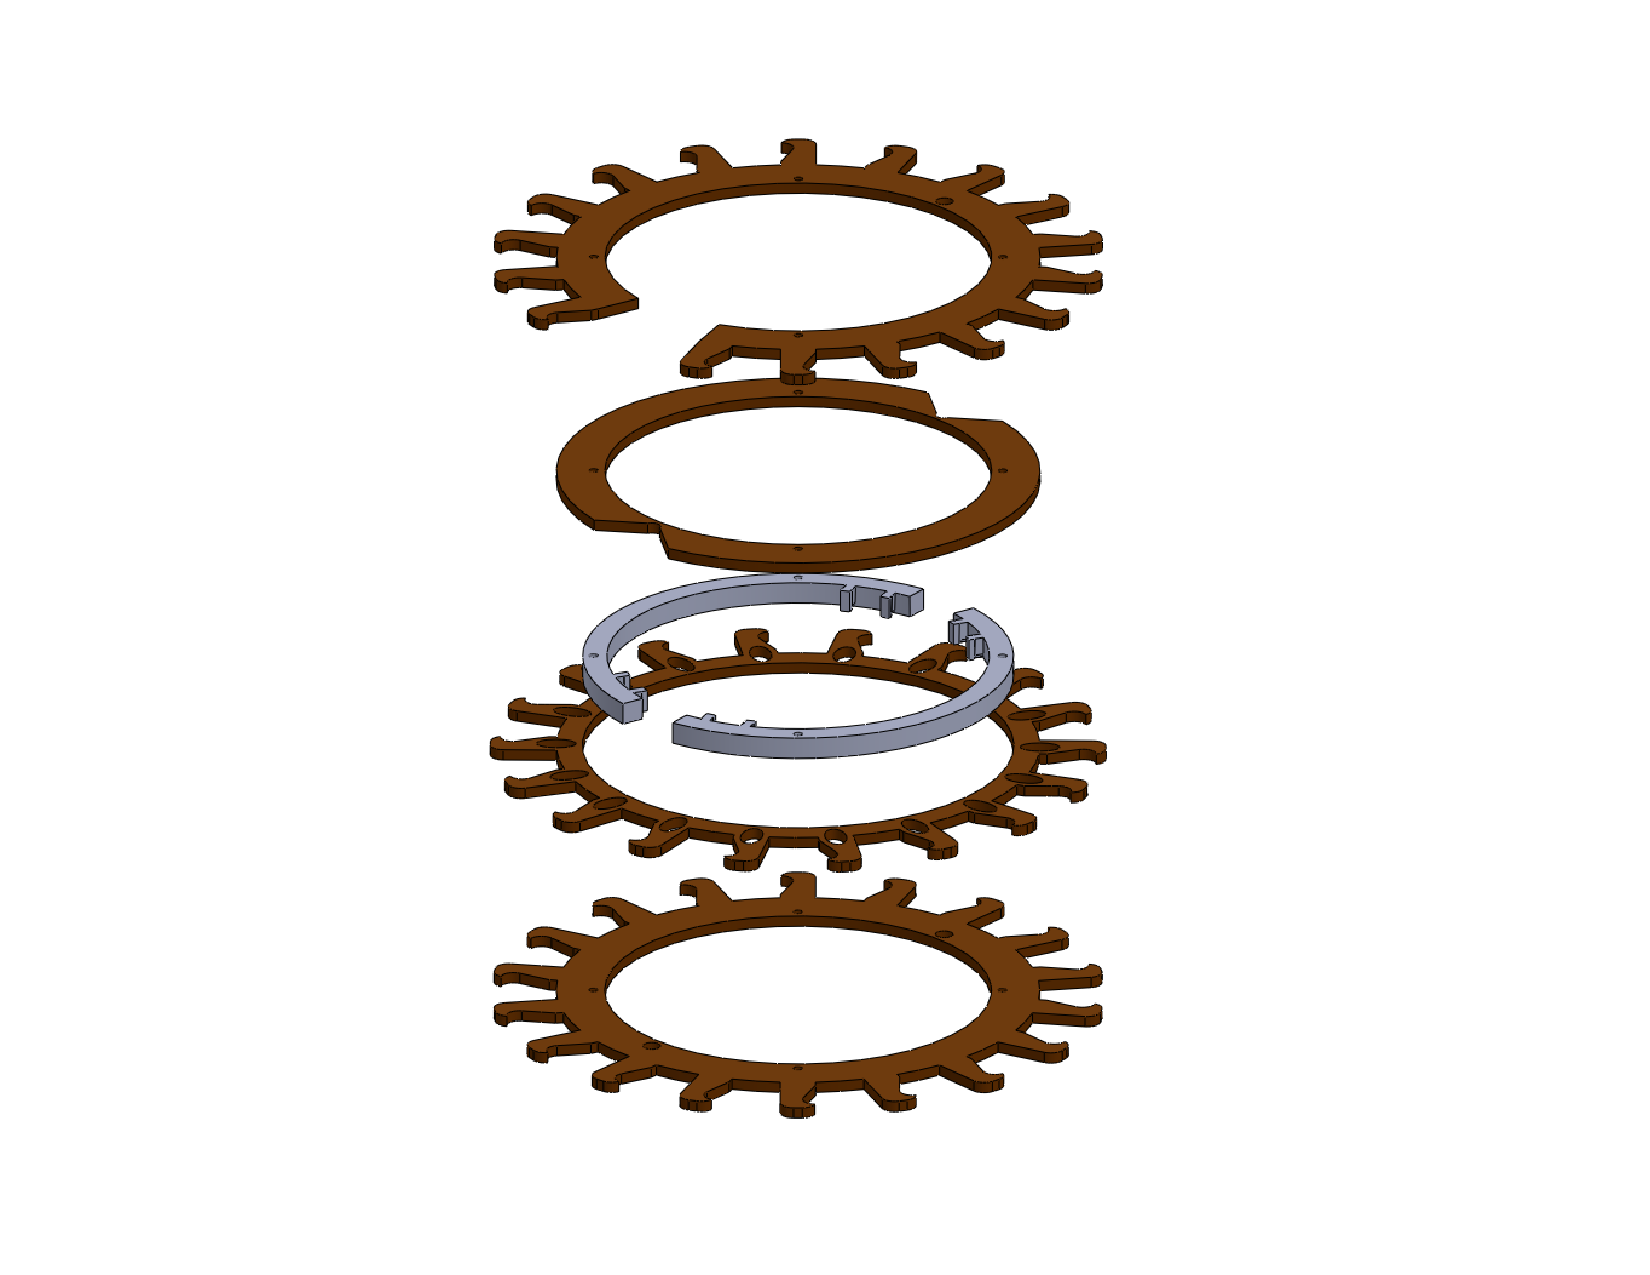
\includegraphics[width=.5\linewidth]{./Figs/final_assembly_explodedisometric.pdf}
\end{center}
\caption{An exploded view of the CAD model of the Actuated Manipulator}
\label{fig:explode}
\end{figure}

As we can see in Figure \ref{fig:explode} that there are five main laser cut components that make up this manipulator. We will start from the top and go to the bottom. The top is a stationary claw with a cutout to allow for the servo. Next is the spacer ring that has cutouts for the servo arm motion. On the prototype, we had to cut out more than the original laser cut-out to allow for the servo arm to rotate, so this will need to be adjusted in the SolidWorks model. Moving down, next comes the mounting clips, which should be already attached to the robot. On the screws, at this point, we installed some spacers (\#4 by 1/8th inch should suffice) Next on, comes the moving ring which fits around the spacers, to prevent lateral movement and isolate the radial movement. Finally, we attached the last stationary ring.
\bf{\sc{Note:}}Be sure to mount the rings so that the stationary claws are mounted in the same direction and a direction opposite to the moving claw.

All of these pieces are attached together with \#2-40x1.25in plastic slotted screws and \#2-40 washers, however the slotted screws can be replaced with metal hex head screws for added support.